\documentclass[11pt,a4paper]{article}
\newcommand{\gls}[1]{#1\textsubscript{G}}
\usepackage[utf8]{inputenc}
\usepackage[italian]{babel}
\usepackage{geometry}
\usepackage{graphicx}
\usepackage{float}
\usepackage{tabularx}
\usepackage{booktabs}
\usepackage{caption}
\usepackage{hyperref}
\usepackage{fancyhdr}
\usepackage{lastpage}

\usepackage{array}
\newcolumntype{M}[1]{>{\centering\arraybackslash}m{#1}}

\geometry{margin=2.5cm}

% Intestazione e piè di pagina
\pagestyle{fancy}
\fancyhf{}
\renewcommand{\headrulewidth}{0pt}
\fancyfoot[C]{\thepage\ di \pageref{LastPage}}

\begin{document}

% Prima pagina - Intestazione
\begin{titlepage}
    \centering
    
    % Logo Università
    \begin{figure}[H]
        \centering
        
\includegraphics[width=0.3\textwidth]{../logoUnipd.jpg}
    \end{figure}
    
    \vspace{0.5cm}
    
    \textbf{\Large Università degli Studi di Padova} \\
    \vspace{0.2cm}
    \textbf{Laurea in Informatica} \\
    \vspace{0.2cm}
    \textbf{Corso di Ingegneria del Software} \\
    \vspace{0.2cm}
    \textbf{Anno Accademico 2025/2026} \\
    
    \vspace{1cm}
    
    % Logo gruppo
    \begin{figure}[H]
        \centering
        
\includegraphics[width=0.2\textwidth]{../LogoByteMe.jpg}
    \end{figure}
    
    \vspace{0.5cm}
    
    \textbf{\Large Gruppo ByteMe} \\
    \vspace{0.2cm}
    \texttt{byteme2025swe@gmail.com} \\
    
    \vspace{1cm}
    
    \textbf{\Huge Piano di Qualifica} \\
    
    \vspace{1.5cm}
    
    \begin{table}[H]
        \centering
        \begin{tabular}{|l|p{5cm}|}
            \hline
            \textbf{Versione} & 1.0.0 \\
            \hline
            \textbf{Stato} & Approvato \\
            \hline
            \textbf{Redazione} & Elisa Marchioro, Giulia Barzon \\
            \hline
            \textbf{\gls{Verifica}} & Elisa Marchioro, Giulia Barzon, Chiara Grossele \\
            \hline
            \textbf{Approvazione} & Joseph Grant \\
            \hline
            \textbf{Proprietario} & ByteMe \\
            \hline
            \textbf{Uso} & Esterno \\
            \hline
            \textbf{Destinatari} & Prof. Tullio Vardanega \\ & Prof. Riccardo Cardin \\
            \hline
        \end{tabular}
    \end{table}
    
    \vfill
\end{titlepage}

% Seconda pagina - Versionamento
\thispagestyle{empty}
\section*{Registro dei Cambiamenti}

\begin{table}[H]
    \centering
    \begin{tabular}{|c|c|c|>{\raggedright\arraybackslash}p{0.35\textwidth}|p{0.18\textwidth}|}
        \hline
        \textbf{Versione} & \textbf{Data} & \textbf{Autore} & \textbf{Descrizione} & \textbf{\gls{Verifica}} \\
        \hline
        1.0.0 & 26/02/2026 & Joseph Grant & Approvazione finale del documento &  \\
        \hline
        0.2.0 & 24/02/2026 & Giulia Barzon & Aggiornamento \gls{cruscotto di qualità} & Elisa Marchioro e Chiara Grossele\\
        \hline
        0.1.5 & 21/02/2026 & Giulia Barzon & Aggiunti test \gls{analisi dinamica} & Elisa Marchioro e Chiara Grossele\\
        \hline
        0.1.4 & 05/02/2026 & Giulia Barzon & Aggiornamento \gls{cruscotto di qualità} & Elisa Marchioro e Chiara Grossele\\
        \hline
        0.1.3 & 11/01/2026 & Elisa Marchioro & Aggiunte metriche qualità di prodotto & Giulia Barzon \\
        \hline
        0.1.2 & 11/01/2026 & Giulia Barzon & Aggiunte metriche qualità di processo & Elisa Marchioro\\
        \hline
        0.1.1 & 27/12/2025 & Joseph Grant & Aggiunta sezione '\gls{verifica}' al \gls{versionamento} & Giulia Barzon\\
        \hline
        0.1.0 & 15/12/2025 & Giulia Barzon & Creazione del documento, scrittura introduzione e \gls{checklist} & Elisa Marchioro\\
        \hline
    \end{tabular}
    \caption{Registro delle versioni del documento}
    \label{tab:versionamento}
\end{table}

\newpage

% Terza pagina - Indice
\tableofcontents
\thispagestyle{empty}
\newpage

\setcounter{page}{1}

\section{Introduzione}

\subsection{Scopo del documento}
Il presente documento ha lo scopo di definire la strategia, le metodologie e le risorse pianificate per garantire la qualità del prodotto software \textbf{"Second Brain"} e l'efficienza dei processi di sviluppo adottati dal gruppo. Esso funge da riferimento principale per le attività di \textbf{\gls{verifica}} (accertamento che il prodotto sia costruito correttamente) e \textbf{\gls{validazione}} (accertamento che il prodotto giusto sia stato costruito), stabilendo gli standard qualitativi che ogni artefatto deve soddisfare prima di essere approvato.
In questo contesto, il termine \textbf{"Qualità"} viene inteso secondo due prospettive complementari:
\begin{itemize}
    \item \textbf{Qualità di processo:} L'aderenza del team al metodo di lavoro definito nelle \textit{\gls{Norme di Progetto}}, basato sul miglioramento continuo e sull'efficienza delle procedure di sviluppo e test.
    \item \textbf{Qualità di prodotto:} La capacità del software di soddisfare i \gls{requisiti funzionali} e non funzionali esplicitati nell'\textit{\gls{Analisi dei Requisiti}}.
\end{itemize}
Il documento è destinato al committente Prof. Vardanega e Prof. Cardin, all'azienda proponente Zucchetti S.p.A. e al gruppo di sviluppo ByteMe.

\subsection{Scopo del prodotto}
Il progetto \textbf{Second Brain}, proposto dall'azienda Zucchetti, mira a sviluppare un \gls{editor di testo} avanzato basato sul linguaggio \gls{MarkDown} e potenziato dall'integrazione di Large Language Models (LLM).
L'applicazione web consentirà all'utente di:
\begin{itemize}
    \item Scrivere e visualizzare in tempo reale testi formattati in \gls{MarkDown};
    \item Interagire con un LLM per generare, riassumere, riscrivere, tradurre e analizzare testi;
    \item Sfruttare il metodo dei "Sei cappelli per pensare" di Edward De Bono per ottenere analisi critiche multi-prospettiche;
    \item Fornire prompt testuali per delegare all'AI la stesura completa del contenuto (\textit{\gls{Distant Writing}}).
\end{itemize}
L'obiettivo è creare uno strumento di supporto alla scrittura creativa e al note-taking avanzato, esplorando le potenzialità pratiche degli LLM nel flusso di lavoro quotidiano.


\subsection{\gls{Glossario}}
Per evitare ambiguità e garantire un linguaggio comune all'interno del gruppo e con i committenti, i termini tecnici utilizzati in questo documento sono definiti in modo approfondito nel documento \textit{\gls{Glossario}}, situato nella \gls{repository} del gruppo alla sezione \textit{Documenti interni}. Per facilitare la lettura, i termini che presentano una definizione specifica nel \gls{glossario} sono contrassegnati con una G a pedice.

\subsection{Riferimenti}
\subsubsection{Riferimenti normativi}
\begin{itemize}
    \item \textbf{Capitolato d'appalto C6:} Second Brain - \textit{Zucchetti}
    \item \textbf{\gls{Norme di Progetto} v1.0.0:} Documento interno del gruppo che definisce regole, strumenti e procedure.
    \item \textbf{Regolamento del progetto didattico:} Corso di Ingegneria del Software, Università degli Studi di Padova.
\end{itemize}

\subsubsection{Riferimenti informativi}
\begin{itemize}
    \item \textbf{ISO/IEC 12207:} \textit{Systems and software engineering — Software life cycle processes}. (Standard di riferimento per il ciclo di vita del software).
    \item \textbf{ISO/IEC 25010:} \textit{Systems and software engineering — Systems and software Quality Requirements and Evaluation (SQuaRE)}. (Modello di riferimento per la qualità del prodotto software).
    \item \textbf{Slide del corso di Ingegneria del Software:}
    \begin{itemize}
        \item T9 - \gls{Verifica} e \gls{validazione}.
        \item T10 - \gls{Analisi statica}.
        \item T11 - \gls{Analisi dinamica}.
    \end{itemize}
    \item \textbf{Slide e dispense del corso opzionale:} \textit{Metodi e Tecnologie per lo Sviluppo Software}.
    \item \textbf{Documentazione tecnica strumenti:} \textit{\gls{GitHub} Actions Documentation}
\end{itemize}

\newpage

\section{Metriche di qualità}
\subsection{Qualità di processo}

\subsubsection{\gls{Processi primari di fornitura}}
In questa sezione vengono definite le metriche relative alla gestione manageriale ed economica del progetto. L'obiettivo è monitorare l'allocazione delle risorse, il rispetto delle scadenze temporali e l'aderenza al preventivo definito in fase di candidatura.
Per garantire un controllo oggettivo sull'avanzamento dei lavori, il gruppo adotta lo standard \textbf{EVA (Earned Value Analysis)\textsubscript{G}}, che permette di integrare la misurazione di tempi, costi e valore prodotto in un unico framework quantitativo.

% PARAMETRI X PROCESSI DI FORNITURA
\paragraph{Budget at Completion\textsubscript{G} (BAC)} \hfill \\
Questo valore indica il budget totale massimo a disposizione del gruppo per lo svolgimento del progetto; rappresenta il limite di spesa totale.

Il preventivo iniziale, calcolato in fase di candidatura, ammonta a \textbf{11.395 euro} per un totale di 558 ore di lavoro.
\begin{itemize}
    \item \textbf{Soglia accettabile}: minimizzato.
    \item \textbf{Soglia ottimale}: minimizzato.
\end{itemize}


\paragraph{Planned Value\textsubscript{G} (PV)} \hfill \\
Valore monetario (o in ore) delle attività pianificate che avrebbero dovuto essere completate entro la data corrente. Si distingue in:
\begin{itemize}
    \item \textbf{\gls{Sprint} Planned Value (SPV)} \\
    Valore pianificato per un singolo \gls{Sprint}. Calcolato come somma delle ore ruolo (OR) preventivate moltiplicate per il costo orario (CR).
    
    \begin{table}[H]
        \centering
        \renewcommand{\arraystretch}{1.5} % Aumenta l'altezza delle righe
        \begin{tabular}{|M{0.4\textwidth}|M{0.25\textwidth}|M{0.25\textwidth}|}
            \hline
            \textbf{Calcolo} & \textbf{Soglia accettabile} & \textbf{Soglia ottimale} \\
            \hline
            $SPV = \sum (OR \times CR)$ & $> 0$ & $> 0$ \\
            \hline
        \end{tabular}
        \caption{Parametro \gls{Sprint} Planned Value (SPV)}
    \end{table}

    \item \textbf{Project Planned Value (PPV)} \\
    Valore pianificato cumulativo per l'intero progetto (somma degli SPV passati).
    
    \begin{table}[H]
        \centering
        \renewcommand{\arraystretch}{1.5} % Aumenta l'altezza delle righe
        \begin{tabular}{|M{0.4\textwidth}|M{0.25\textwidth}|M{0.25\textwidth}|}
            \hline
            \textbf{Calcolo} & \textbf{Soglia accettabile} & \textbf{Soglia ottimale} \\
            \hline
            $PPV = \sum SPV_{passati}$ & $> 0$ & $> 0$ \newline $\le BAC$ \\
            \hline
        \end{tabular}
        \caption{Parametro Project Planned Value (PPV)}
    \end{table}
\end{itemize}


\paragraph{Actual Cost\textsubscript{G} (AC)} \hfill \\
Costo effettivo sostenuto (ore lavorate $\times$ costo orario) per il lavoro svolto finora. Si distingue in:

\begin{itemize}
    \item \textbf{\gls{Sprint} Actual Cost (SAC)} \\
    Costo sostenuto nel singolo \gls{Sprint}.
    
    \begin{table}[H]
        \centering
        \renewcommand{\arraystretch}{1.5} % Aumenta l'altezza delle righe
        \begin{tabular}{|M{0.4\textwidth}|M{0.25\textwidth}|M{0.25\textwidth}|}
            \hline
            \textbf{Calcolo} & \textbf{Soglia accettabile} & \textbf{Soglia ottimale} \\
            \hline
            $SAC = \sum \textrm{costi sostenuti nello \gls{Sprint}}$ & $\le SPV + 10\%$ & $\le SPV$ \\
            \hline
        \end{tabular}
        \caption{Parametro \gls{Sprint} Actual Cost (SAC)}
    \end{table}

    \item \textbf{Project Actual Cost (PAC)} \\
    Costo totale sostenuto dall'inizio del progetto.

    \begin{table}[H]
        \centering
        \renewcommand{\arraystretch}{1.5} % Aumenta l'altezza delle righe
        \begin{tabular}{|M{0.4\textwidth}|M{0.25\textwidth}|M{0.25\textwidth}|}
            \hline
            \textbf{Calcolo} & \textbf{Soglia accettabile} & \textbf{Soglia ottimale} \\
            \hline
            $PAC = \sum_{s \in S} SAC_s$ & $\le BAC$ & $\le BAC$ \\
            \hline
        \end{tabular}
        \caption{Parametro Project Actual Cost (PAC)}
    \end{table}
\end{itemize}


\paragraph{Earned Value\textsubscript{G} (EV)} \hfill \\
Rappresenta il valore del lavoro effettivamente completato e verificato alla data corrente. Per calcolarlo si adotta la tecnica di misurazione fisica \textbf{0/100}\textsubscript{G}: il valore pianificato di un'attività viene accreditato solo se l'attività è completata al 100\%.

\begin{itemize}
    \item \textbf{\gls{Sprint} Earned Value (SEV)} \\
    Valore guadagnato nel singolo \gls{Sprint}. È la somma del Planned Value delle sole attività completate secondo la Definition of Done.
    
    \begin{table}[H]
        \centering
        \renewcommand{\arraystretch}{1.5}
        \begin{tabular}{|M{0.4\textwidth}|M{0.25\textwidth}|M{0.25\textwidth}|}
            \hline
            \textbf{Calcolo} & \textbf{Soglia accettabile} & \textbf{Soglia ottimale} \\
            \hline
            $SEV = \sum PV_{completati}$ & $\ge 90\%$ del SPV & $= SPV$ \\
            \hline
        \end{tabular}
        \caption{Parametro \gls{Sprint} Earned Value (SEV)}
    \end{table}

    \item \textbf{Project Earned Value (PEV)} \\
    Valore guadagnato cumulativo dall'inizio del progetto.
    
    \begin{table}[H]
        \centering
        \renewcommand{\arraystretch}{1.5}
        \begin{tabular}{|M{0.4\textwidth}|M{0.25\textwidth}|M{0.25\textwidth}|}
            \hline
            \textbf{Calcolo} & \textbf{Soglia accettabile} & \textbf{Soglia ottimale} \\
            \hline
            $PEV = \sum SEV_{passati}$ & $\ge 90\%$ del PPV & $= PPV$ \\
            \hline
        \end{tabular}
        \caption{Parametro Project Earned Value (PEV)}
    \end{table}
\end{itemize}


% INIZIO METRICHE FORNITURA
\paragraph{Schedule Variance\textsubscript{G} (SV)} \hfill \\
Misura lo scostamento temporale del progetto rispetto alla pianificazione iniziale. Indica se il progetto è in anticipo, in pari o in ritardo in termini di valore prodotto.

\begin{table}[H]
    \centering
    \renewcommand{\arraystretch}{1.5} % Spaziatura aumentata
    \begin{tabular}{|M{0.4\textwidth}|M{0.25\textwidth}|M{0.25\textwidth}|}
        \hline
        \textbf{Calcolo} & \textbf{Soglia accettabile} & \textbf{Soglia ottimale} \\
        \hline
        $SV = EV - PV$ & $SV \ge -10\%$ del PV & $SV \ge 0$ \\
        \hline
    \end{tabular}
    \caption{Metrica Schedule Variance (SV)}
\end{table}

\paragraph{Cost Variance\textsubscript{G} (CV)} \hfill \\
Misura l'efficienza economica del progetto, confrontando il valore prodotto (guadagnato) con i costi effettivamente sostenuti. Indica se stiamo spendendo più del necessario per il lavoro svolto.

\begin{table}[H]
    \centering
    \renewcommand{\arraystretch}{1.5} % Spaziatura aumentata
    \begin{tabular}{|M{0.4\textwidth}|M{0.25\textwidth}|M{0.25\textwidth}|}
        \hline
        \textbf{Calcolo} & \textbf{Soglia accettabile} & \textbf{Soglia ottimale} \\
        \hline
        $CV = EV - AC$ & $CV \ge -8\%$ del EV & $CV \ge 0$ \\
        \hline
    \end{tabular}
    \caption{Metrica Cost Variance (CV)}
\end{table}

\paragraph{Cost Performance Index\textsubscript{G} (CPI)} \hfill \\
Indice di efficienza dei costi. Rapporto tra il valore guadagnato e il costo effettivo sostenuto. Un valore inferiore a 1 indica che il costo sostenuto è superiore al valore prodotto.

\begin{table}[H]
    \centering
    \renewcommand{\arraystretch}{1.5}
    \begin{tabular}{|M{0.4\textwidth}|M{0.25\textwidth}|M{0.25\textwidth}|}
        \hline
        \textbf{Calcolo} & \textbf{Soglia accettabile} & \textbf{Soglia ottimale} \\
        \hline
        $CPI = \frac{PEV}{PAC}$ & $CPI \ge 0.95$ & $CPI \ge 1.00$ \\
        \hline
    \end{tabular}
    \caption{Metrica Cost Performance Index (CPI)}
\end{table}

\paragraph{Schedule Performance Index\textsubscript{G} (SPI)} \hfill \\
Indice di efficienza temporale; è il rapporto tra il valore guadagnato e il valore pianificato. Indica la velocità di avanzamento rispetto al piano.

\begin{table}[H]
    \centering
    \renewcommand{\arraystretch}{1.5}
    \begin{tabular}{|M{0.4\textwidth}|M{0.25\textwidth}|M{0.25\textwidth}|}
        \hline
        \textbf{Calcolo} & \textbf{Soglia accettabile} & \textbf{Soglia ottimale} \\
        \hline
        $SPI = \frac{EV}{PV}$ & $SPI \ge 0.90$ & $SPI \ge 1.00$ \\
        \hline
    \end{tabular}
    \caption{Metrica Schedule Performance Index (SPI)}
\end{table}

\paragraph{Estimated at Completion\textsubscript{G} (EAC)} \hfill \\
Stima aggiornata del costo totale finale del progetto, calcolata proiettando l'efficienza attuale (CPI) fino alla fine del progetto.

\begin{table}[H]
    \centering
    \renewcommand{\arraystretch}{1.5}
    \begin{tabular}{|M{0.4\textwidth}|M{0.25\textwidth}|M{0.25\textwidth}|}
        \hline
        \textbf{Calcolo} & \textbf{Soglia accettabile} & \textbf{Soglia ottimale} \\
        \hline
        $EAC = \frac{BAC}{CPI}$ & $EAC \le BAC$ & $EAC \le BAC$ \\
        \hline
    \end{tabular}
    \caption{Metrica Estimated at Completion (EAC)}
\end{table}

\newpage
\subsubsection{\gls{Processi primari di sviluppo}}
Questa sezione raggruppa le metriche utilizzate per valutare la qualità delle attività di realizzazione tecnica del prodotto.
Il monitoraggio si focalizza sulla \textbf{stabilità dei requisiti}, per controllare l'evoluzione dello scopo del progetto ed evitare cambiamenti incontrollati, e sulla \textbf{qualità strutturale del codice}, analizzando la complessità e la dimensione del software prodotto per garantirne la manutenibilità futura.

\paragraph{Requirements Stability Index\textsubscript{G} (RSI)} \hfill \\
Misura la stabilità dei requisiti nel corso del tempo, indicando la percentuale di requisiti rimasti invariati rispetto al totale. Un valore basso indica frequenti cambiamenti nello scopo del progetto.

\begin{table}[H]
    \centering
    \renewcommand{\arraystretch}{1.5}
    \begin{tabular}{|M{0.4\textwidth}|M{0.25\textwidth}|M{0.25\textwidth}|}
        \hline
        \textbf{Calcolo} & \textbf{Soglia accettabile} & \textbf{Soglia ottimale} \\
        \hline
        $RSI = (1 - \frac{N_{modifiche}}{N_{totali}}) \times 100$ & $RSI \ge 80\%$ & $RSI = 100\%$ \\
        \hline
    \end{tabular}
    \caption{Metrica Requirements Stability Index (RSI)}
\end{table}

\paragraph{Copertura dei Requisiti\textsubscript{G} (CR)} \hfill \\
Percentuale di requisiti implementati e verificati (soddisfatti) rispetto al totale pianificato, suddivisi per importanza (Obbligatori, Desiderabili, Opzionali).

\begin{table}[H]
    \centering
    \renewcommand{\arraystretch}{1.5}
    \begin{tabular}{|M{0.4\textwidth}|M{0.25\textwidth}|M{0.25\textwidth}|}
        \hline
        \textbf{Calcolo} & \textbf{Soglia accettabile} & \textbf{Soglia ottimale} \\
        \hline
        $C = \frac{N_{soddisfatti}}{N_{totali}} \times 100$ & 
        Obbl: $100\%$ \newline Desid: $\ge 40\%$ \newline Opz: $\ge 0\%$ & 
        Obbl: $100\%$ \newline Desid: $100\%$ \newline Opz: $100\%$ \\
        \hline
    \end{tabular}
    \caption{Metrica Copertura dei Requisiti (CR)}
\end{table}

\paragraph{Lines of Code\textsubscript{G} (LOC)} \hfill \\
Misura la dimensione fisica del software tramite il conteggio delle righe di codice sorgente (esclusi commenti e righe vuote). Questa è una metrica informativa di monitoraggio, quindi non vengono valutate le soglie.

\begin{table}[H]
    \centering
    \renewcommand{\arraystretch}{1.5}
    \begin{tabular}{|M{0.4\textwidth}|M{0.25\textwidth}|M{0.25\textwidth}|}
        \hline
        \textbf{Calcolo} & \textbf{Soglia accettabile} & \textbf{Soglia ottimale} \\
        \hline
        Somma righe logiche nei file sorgente & N/A & N/A \\
        \hline
    \end{tabular}
    \caption{Metrica Lines of Code (LOC)}
\end{table}

\paragraph{Complessità Ciclomatica\textsubscript{G} (McCabe)} \hfill \\
Misura la complessità del flusso di controllo di un metodo o funzione calcolando il numero di cammini linearmente indipendenti. Una complessità elevata indica codice difficile da testare e mantenere.

\begin{table}[H]
    \centering
    \renewcommand{\arraystretch}{1.5}
    \begin{tabular}{|M{0.4\textwidth}|M{0.25\textwidth}|M{0.25\textwidth}|}
        \hline
        \textbf{Calcolo} & \textbf{Soglia accettabile} & \textbf{Soglia ottimale} \\
        \hline
        $v(G) = E - N + 2P$ & $\le 8$ & $\le 6$ \\
        \hline
    \end{tabular}
    \caption{Metrica Complessità Ciclomatica (McCabe)}
\end{table}

\newpage
\subsubsection{\gls{Processi di supporto}: documentazione e qualità}
Le metriche esposte in questa sezione valutano l'\gls{efficacia} delle attività trasversali che supportano il ciclo di vita del software.
L'attenzione è posta sulla \textbf{qualità della documentazione}, assicurando che sia leggibile, corretta e priva di ambiguità, e sull'\gls{efficacia} del \textbf{processo di \gls{verifica}}, misurando la capacità del gruppo di identificare e risolvere rischi e difetti in modo proattivo.

\paragraph{Indice di Gulpease\textsubscript{G} (IG)} \hfill \\
Valuta la leggibilità di un testo redatto in lingua italiana per garantire che la documentazione sia comprensibile ai membri del gruppo e agli stakeholder esterni.

\begin{table}[H]
    \centering
    \renewcommand{\arraystretch}{1.5}
    \begin{tabular}{|M{0.4\textwidth}|M{0.25\textwidth}|M{0.25\textwidth}|}
        \hline
        \textbf{Calcolo} & \textbf{Soglia accettabile} & \textbf{Soglia ottimale} \\
        \hline
        $IG = 89 + \frac{300 \times N_{frasi} - 10 \times N_{lettere}}{N_{parole}}$ & $G \ge 40$ & $G \ge 60$ \\
        \hline
    \end{tabular}
    \caption{Metrica Indice di Gulpease (IG)}
\end{table}

\paragraph{Correttezza Ortografica (CO)} \hfill \\
Misura il numero di errori ortografici o grammaticali residui nei documenti individuati durante i processi di \gls{verifica} o revisione.

\begin{table}[H]
    \centering
    \renewcommand{\arraystretch}{1.5}
    \begin{tabular}{|M{0.4\textwidth}|M{0.25\textwidth}|M{0.25\textwidth}|}
        \hline
        \textbf{Calcolo} & \textbf{Soglia accettabile} & \textbf{Soglia ottimale} \\
        \hline
        Conteggio errori manuale/tool & 0 & 0 \\
        \hline
    \end{tabular}
    \caption{Metrica Correttezza Ortografica (CO)}
\end{table}

\paragraph{Rischi Non Calcolati (RNC)} \hfill \\
Quantità di rischi che si verificano durante il progetto ma che non erano stati previsti o analizzati in fase di candidatura e nel documento Piano di Progetto.

\begin{table}[H]
    \centering
    \renewcommand{\arraystretch}{1.5}
    \begin{tabular}{|M{0.4\textwidth}|M{0.25\textwidth}|M{0.25\textwidth}|}
        \hline
        \textbf{Calcolo} & \textbf{Soglia accettabile} & \textbf{Soglia ottimale} \\
        \hline
        Conteggio rischi imprevisti & $\le 2$ & $0$ \\
        \hline
    \end{tabular}
    \caption{Metrica Rischi Non Calcolati (RNC)}
\end{table}

\paragraph{Metriche Soddisfatte (MS)} \hfill \\
Percentuale di metriche (tra tutte quelle definite nel presente documento) che rientrano nelle soglie di accettabilità ad ogni \gls{verifica} di periodo. Indica lo stato di salute generale del progetto.

\begin{table}[H]
    \centering
    \renewcommand{\arraystretch}{1.5}
    \begin{tabular}{|M{0.4\textwidth}|M{0.25\textwidth}|M{0.25\textwidth}|}
        \hline
        \textbf{Calcolo} & \textbf{Soglia accettabile} & \textbf{Soglia ottimale} \\
        \hline
        $MS = \frac{metricheOK}{TOTmetriche} \times 100$ & $\ge 75\%$ & $100\%$ \\
        \hline
    \end{tabular}
    \caption{Metrica Metriche Soddisfatte (MS)}
\end{table}


\newpage
\subsection{Qualità di prodotto}
La qualità di prodotto nel software indica quanto bene un sistema riesce a soddisfare i bisogni degli utenti e gli obiettivi per cui è stato creato. Non significa solo che il programma funzioni, ma anche che sia affidabile, veloce, facile da usare e capace di essere migliorato nel tempo. Un software di buona qualità è quindi utile, stabile e adatto a evolversi insieme alle esigenze degli utenti.
\subsubsection{\gls{Adeguatezza funzionale}}
Indica quanto il software realizza correttamente tutte le funzioni richieste per soddisfare gli obiettivi dell’utente.
\begin{table}[H]
\centering
\renewcommand{\arraystretch}{1.5}
\begin{tabular}{|M{0.25\textwidth}|M{0.35\textwidth}|M{0.15\textwidth}|M{0.15\textwidth}|}
\hline
\textbf{Metrica} & \textbf{Scopo della metrica} & \textbf{Soglia accettabile} & \textbf{Soglia ottimale} \\
\hline
Requirement Coverage & \gls{Verifica} che tutte le funzionalità principali dell’editor siano implementate & 90\% & 98\% \\ \hline
Acceptance Test Pass Rate & Controlla che le funzionalità principali funzionino correttamente & 95\% & 99\% \\ \hline
Functional Defect Density & Misura quanti bug ci sono per funzione principale & 0.5 bug/funzione & 0.1 bug/funzione \\
\hline
\end{tabular}
\caption{Soglie metriche funzionalità del prodotto}
\end{table}

\subsubsection{\gls{Qualità dell'output generativo}}
Misura quanto le risposte prodotte dal sistema sono corrette, coerenti e utili per l’utente.
\begin{table}[H]
\centering
\renewcommand{\arraystretch}{1.5}
\begin{tabular}{|M{0.25\textwidth}|M{0.35\textwidth}|M{0.15\textwidth}|M{0.15\textwidth}|}
\hline
\textbf{Metrica} & \textbf{Scopo della metrica} & \textbf{Soglia accettabile} & \textbf{Soglia ottimale} \\
\hline
Accuracy & Misura quanto i suggerimenti o correzioni AI sono corretti & 85\% & 95\% \\ \hline
Hallucination Rate & Misura quanto l’AI suggerisce contenuti errati o inventati & 10\% & 2\% \\ \hline
Human Rating & Valutazione soggettiva della qualità dei suggerimenti AI da parte degli utenti & 3.5 / 5 & 4.5 / 5 \\ \hline
Completion Success Rate & Percentuale di suggerimenti AI accettati dall’utente & 75\% & 90\% \\
\hline
\end{tabular}
\caption{Soglie metriche qualità output AI}
\end{table}

\subsubsection{Affidabilità\textsubscript{G}}
Rappresenta la capacità del software di funzionare in modo stabile e continuo senza guasti frequenti.
\begin{table}[H]
\centering
\renewcommand{\arraystretch}{1.5}
\begin{tabular}{|M{0.25\textwidth}|M{0.35\textwidth}|M{0.15\textwidth}|M{0.15\textwidth}|}
\hline
\textbf{Metrica} & \textbf{Scopo della metrica} & \textbf{Soglia accettabile} & \textbf{Soglia ottimale} \\
\hline
Availability & Percentuale di tempo in cui il software è operativo e stabile & 99\% & 99.9\% \\ \hline
Error Rate & Percentuale di operazioni che falliscono (salvataggio, apertura file, AI) & 1\% & 0.1\% \\ \hline
MTTR & Tempo medio per ripristinare il software dopo un crash & 60 minuti & 10 minuti \\
\hline
\end{tabular}
\caption{Soglie metriche affidabilità del prodotto}
\end{table}

\subsubsection{Efficienza\textsubscript{G}}
Indica quanto il sistema è veloce e quanto bene utilizza le risorse disponibili.
\begin{table}[H]
\centering
\renewcommand{\arraystretch}{1.5}
\begin{tabular}{|M{0.25\textwidth}|M{0.35\textwidth}|M{0.15\textwidth}|M{0.15\textwidth}|}
\hline
\textbf{Metrica} & \textbf{Scopo della metrica} & \textbf{Soglia accettabile} & \textbf{Soglia ottimale} \\
\hline
Response Time (Latenza interfaccia) & Tempo medio che l'interfaccia impiega per aggiornarsi correttamente & 500 ms & 100 ms \\ \hline
AI Processing Time & Tempo medio necessario all’AI per generare un testo & 10 sec & 3 sec \\
\hline
\end{tabular}
\caption{Soglie metriche efficienza del prodotto}
\end{table}

\subsubsection{Usabilità\textsubscript{G}}
Descrive quanto il software è facile da imparare e da usare per gli utenti.
\begin{table}[H]
\centering
\renewcommand{\arraystretch}{1.5}
\begin{tabular}{|M{0.25\textwidth}|M{0.35\textwidth}|M{0.15\textwidth}|M{0.15\textwidth}|}
\hline
\textbf{Metrica} & \textbf{Scopo della metrica} & \textbf{Soglia accettabile} & \textbf{Soglia ottimale} \\
\hline
Task Success Rate & Percentuale di utenti che completano correttamente un compito (scrittura, salvataggio, uso AI) & 80\% & 95\% \\ \hline
SUS Score & Valutazione dell’usabilità tramite questionario standard & 68 & 85 \\ \hline
User Satisfaction Rate & Percentuale di utenti soddisfatti delle funzioni AI & 75\% & 90\% \\
\hline
\end{tabular}
\caption{Soglie metriche usabilità del prodotto}
\end{table}

\subsubsection{Manutenibilità\textsubscript{G}}
Indica quanto è semplice correggere, modificare ed evolvere il software nel tempo.
\begin{table}[H]
\centering
\renewcommand{\arraystretch}{1.5}
\begin{tabular}{|M{0.25\textwidth}|M{0.35\textwidth}|M{0.15\textwidth}|M{0.15\textwidth}|}
\hline
\textbf{Metrica} & \textbf{Scopo della metrica} & \textbf{Soglia accettabile} & \textbf{Soglia ottimale} \\
\hline
Test Coverage & Percentuale di codice coperto dai test (funzioni base + AI) & 70\% & 90\% \\ \hline
Change Failure Rate & Percentuale di modifiche che introducono problemi o bug & 15\% & 5\% \\
\hline
\end{tabular}
\caption{Soglie metriche manutenibilità del prodotto}
\end{table}

\newpage
\section{Strategia di \gls{verifica} (Testing)}
\subsection{\gls{Analisi statica}}

\subsubsection{\gls{Checklist} per la \gls{verifica} (\gls{Analisi statica} tramite inspection\textsubscript{G})}
Questa sezione contiene le liste di controllo che i Verificatori devono utilizzare obbligatoriamente prima di approvare un documento o un pezzo di codice. L'obiettivo è standardizzare il controllo qualità ed evitare errori ricorrenti.
Questa \gls{checklist} viene aggiornata progressivamente dai verificatori e permette di evitare gli errori più comuni e semplici da individuare.

% tabella checklist documenti
\begin{table}[H]
    \centering
    \renewcommand{\arraystretch}{1.4}
    \begin{tabular}{|l|>{\raggedright\arraybackslash}p{0.35\textwidth}|>{\raggedright\arraybackslash}p{0.4\textwidth}|}
        \hline
        \textbf{Oggetto} & \textbf{Errore} & \textbf{Azione correttiva} \\
        \hline
        Immagini e tabelle & Mancanza di didascalia (caption) & Ogni tabella o immagine deve avere una didascalia esplicativa numerata. \\
        \hline
        Struttura & Sezioni vuote o orfane & Rimuovere o riempire le sezioni che contengono solo il titolo senza testo. \\
        \hline
        \gls{Glossario} & Termine non marcato o errato & Verificare che i termini del \gls{glossario} siano segnati con la "G" a pedice e rispettino il case sensitivity. \\
        \hline
        Ortografia & Errori di battitura o sintassi & Utilizzare il correttore automatico, verificare personalmente i testi, rimuovere refusi e doppi spazi. \\
        \hline
        Percorsi File & Path immagini errato & Verificare che i percorsi siano relativi e corretti (es: \texttt{../UCimg/diagramma.jpg} per i diagrammi, \texttt{../logo.jpg} per i loghi) per evitare errori di compilazione.\\
        \hline
        \gls{Versionamento} & Disallineamento versione & Controllare che la versione indicata nel frontespizio coincida con l'ultima voce del registro delle modifiche. \\
        \hline
        \gls{Versionamento} & Nome file senza versione & Il nome del documento deve contenere il numero di versione corrente (es. \texttt{Nome\_doc\_v1.0.0}). \\
        \hline
    \end{tabular}
    \caption{\gls{Checklist} documentazione (LaTeX)}
\end{table}

% tabella checklist Codice e Push 
\begin{table}[H]
    \centering
    \renewcommand{\arraystretch}{1.4}
    \begin{tabular}{|l|>{\raggedright\arraybackslash}p{0.35\textwidth}|>{\raggedright\arraybackslash}p{0.4\textwidth}|}
        \hline
        \textbf{Oggetto} & \textbf{Errore} & \textbf{Azione correttiva} \\
        \hline
        Sincronizzazione & Push senza pull & Eseguire sempre \texttt{\gls{git} pull} prima di \texttt{\gls{git} push} per risolvere conflitti locali ed evitare \gls{merge} complessi. \\
        \hline
        Pulizia & Codice commentato o morto & Rimuovere blocchi di codice commentato inutile o funzioni non utilizzate prima del push. \\
        \hline
    \end{tabular}
    \caption{\gls{Checklist} codice e push (\gls{Git})}
\end{table}

% tabella checklist analisi dei requisiti
\begin{table}[H]
    \centering
    \renewcommand{\arraystretch}{1.4}
    \begin{tabular}{|l|>{\raggedright\arraybackslash}p{0.35\textwidth}|>{\raggedright\arraybackslash}p{0.4\textwidth}|}
        \hline
        \textbf{Oggetto} & \textbf{Errore} & \textbf{Azione correttiva} \\
        \hline
        Tracciamento & Requisiti per un caso d'uso assenti & Ad ogni caso d'uso deve corrispondere almeno un requisito. \\
        \hline
        Diagrammi & Diagrammi dei casi d'uso erronei & I diagrammi devono riportare la corretta numerazione e nomenclatura del caso d'uso. \\
        \hline
        Tracciamento & Caso d'uso senza requisiti & Ogni Caso d'Uso (UC) deve generare almeno un Requisito. \\
        \hline
        UML & Inconsistenza diagrammi & La numerazione e i nomi negli schemi UML devono corrispondere esattamente al testo descrittivo. \\
        \hline
        Attori & Attori non definiti & Verificare che tutti gli attori (es. Utente, \gls{Sistema AI}) siano descritti nella sezione introduttiva degli UC. \\
        \hline
        Nomenclatura & Codice identificativo errato & Ogni requisito deve avere un codice univoco che segue la nomenclatura standard definita. \\
        \hline
    \end{tabular}
    \caption{\gls{Checklist} \gls{Analisi Dei Requisiti}}
\end{table}

% SEZIONE PER ANALISI DINAMICA: test implementati sul codice
\newpage
\subsection{\gls{Analisi dinamica}}
L'\gls{analisi dinamica} del software \textit{Second Brain} viene condotta attraverso l'esecuzione di test strutturati su diversi livelli di granularità, secondo il modello a V del ciclo di vita del software. L'obiettivo è verificare che il sistema soddisfi i \gls{requisiti funzionali} e non funzionali, garantendo affidabilità, correttezza e usabilità del prodotto finale.

\paragraph{Priorità di testing (per la fase RTB)}
Durante lo sviluppo del Proof of Concept (PoC), l'\gls{analisi dinamica} si concentra sulla \gls{verifica} della fattibilità tecnologica e sull'integrazione tra i componenti. Le priorità sono così definite:
\begin{itemize}
    \item \textbf{Alta}: \gls{Test di sistema} (funzionalità AI core) e \gls{test di integrazione} (\gls{API} Auth + AI, Backend-\gls{Database}).
    \item \textbf{Media}: Test di unità (logiche isolate come \texttt{auth.py} o formattazione dei prompt).
\end{itemize}
L'obiettivo attuale non è raggiungere una \textit{Code Coverage} esaustiva (che sarà centrale nella fase PB), ma validare che i rischi tecnologici siano stati mitigati.

% ----------------------------------------------------
% TEST DI UNITA'
% ----------------------------------------------------
\subsubsection{Test di unità\textsubscript{G}}
\textbf{Obiettivo}: Verificare il corretto funzionamento delle singole unità software in isolamento (funzioni, metodi, moduli), assicurando che producano l'output atteso per ogni input fornito.

\begin{table}[H]
    \centering
    \small % Carattere leggermente ridotto per far stare tutte le colonne
    \begin{tabularx}{\textwidth}{|c|c|X|p{2.5cm}|p{2.5cm}|}
        \hline
        \textbf{Test ID} & \textbf{Funzione testata} & \textbf{Descrizione} & \textbf{Input} & \textbf{Output atteso} \\
        \hline
        TU-1 & \texttt{genera\_hash()} & \gls{Verifica} generazione hash PBKDF2 con salt casuale. & pwd: "test123" & Stringa formato \texttt{salt\$hash} \\
        \hline
        TU-2 & \texttt{\gls{verifica}\_pwd()} & \gls{Verifica} confronto con una password corretta. & pwd: "test123", hash valido & \texttt{True} \\
        \hline
        TU-3 & \texttt{\gls{verifica}\_pwd()} & \gls{Verifica} rifiuto con una password errata. & pwd: "wrong", hash valido & \texttt{False} \\
        \hline
        TU-4 & \texttt{\gls{verifica}\_pwd()} & Gestione delle eccezioni per hash malformati o nulli. & hash malformato & \texttt{False} \\
        \hline
    \end{tabularx}
    \caption{Test di unità}
\end{table}

% ----------------------------------------------------
% TEST DI INTEGRAZIONE
% ----------------------------------------------------
\subsubsection{\gls{Test di integrazione}}
\textbf{Obiettivo}: Verificare che i diversi moduli del sistema (Frontend, Backend, \gls{Database} e LLM esterni) comunichino correttamente tra loro attraverso le rispettive interfacce e \gls{API}.

\begin{table}[H]
    \centering
    \small
    \begin{tabularx}{\textwidth}{|c|X|c|}
        \hline
        \textbf{Test ID} & \textbf{Descrizione} & \textbf{Requisito} \\
        \hline
        TI-1 & \textbf{Health Check \gls{Database}}: \gls{Verifica} che il backend riesca a stabilire una connessione stabile con il \gls{database} \gls{PostgreSQL} interrogando l'\gls{endpoint} dedicato (\texttt{/\gls{api}/test-db-connection}) ed eseguendo una query di test. & ROP-F-22 \\
        \hline
        TI-2 & \textbf{Health Check LLM}: \gls{Verifica} in fase di avvio dell'applicazione che le variabili d'ambiente (\gls{API} Key e Base URL) siano correttamente caricate e che il client verso il provider esterno venga inizializzato con successo. & RO-V-13 \\
        \hline
        TI-3 & \gls{Verifica} che la chiamata di registrazione dal backend salvi correttamente e persistentemente il record del nuovo utente all'interno del \gls{database} \gls{PostgreSQL}. & ROP-F-11 \\
        \hline
        TI-4 & \gls{Verifica} che l'\gls{endpoint} del backend formatti correttamente il prompt richiesto e lo inoltri con successo alle \gls{API} del provider LLM, ricevendo una risposta valida. & RO-V-13 \\
        \hline
        TI-5 & \gls{Verifica} che la funzione frontend \texttt{loginUtente()} componga correttamente il body JSON della richiesta HTTP POST e gestisca adeguatamente la risposta del backend (es. token di sessione o errore). & ROP-F-9 \\
        \hline
    \end{tabularx}
    \caption{\gls{Test di integrazione}}
\end{table}

% ----------------------------------------------------
% TEST DI SISTEMA
% ----------------------------------------------------
\subsubsection{\gls{Test di sistema}}
\textbf{Obiettivo}: Validare il comportamento del software nel suo complesso, simulando i percorsi d'uso (End-to-End) dell'utente finale tramite l'interfaccia grafica per garantire la copertura dei casi d'uso.

\begin{table}[H]
    \centering
    \small
    \begin{tabularx}{\textwidth}{|c|X|c|}
        \hline
        \textbf{Test ID} & \textbf{Descrizione} & \textbf{Caso d'Uso (UC)} \\
        \hline
        TS-1 & \textbf{Flusso autenticazione}: L'utente accede alla pagina di login, inserisce credenziali valide e preme "Accedi". Il sistema lo reindirizza all'editor, nasconde i bottoni di login/registrazione e l'area utente. & UC-5.0, UC-5.5 \\
        \hline
        TS-2 & \textbf{Flusso AI core}: L'utente carica un file locale, ne seleziona una porzione, richiede un'operazione all'AI (es. "Riassumi"). Il sistema elabora la richiesta e inietta il risultato nel pannello "Storico Generazioni". & UC-2.* \\
        \hline
        TS-3 & \textbf{Flusso editor e I/O}: L'utente scrive testo formattato in \gls{Markdown} nell'editor, \gls{verifica} che la sintassi venga riconosciuta, ed esegue il salvataggio (download) del file in formato .md sul proprio dispositivo. & UC-1.0, UC-4.0 \\
        \hline
    \end{tabularx}
    \caption{\gls{Test di sistema}}
\end{table}

% \subsubsection{Test di Accettazione\textsubscript{G}}

\newpage
\section{Cruscotto di valutazione della qualità}
In questa sezione vengono presentati gli indicatori di qualità relativi al processo produttivo, al fine di valutarne l'andamento durante le due fasi di progetto: RTB (Requirements and Technology Baseline) e PB (Product Baseline).

\subsection{Qualità di processo}

\subsubsection{Estimated at Completion (EAC)}
% [GRAFICO DELL'ANDAMENTO EAC]
\begin{figure}[H]
    \centering
    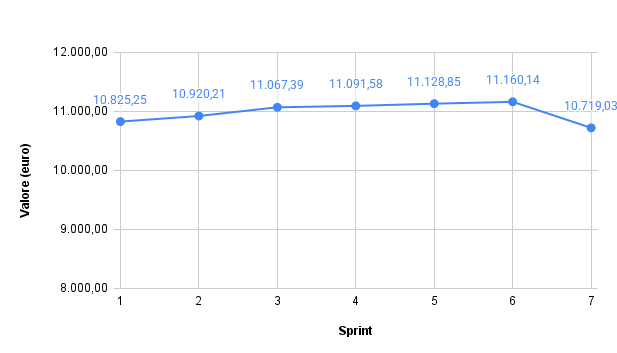
\includegraphics[width=0.75\textwidth]{../graficiMetriche/EAC.png}
    \caption{Andamento del valore di Estimated at Completion (EAC) nella fase RTB}
\end{figure}

\textbf{RTB:} L'analisi dell'Estimated at Completion (EAC) mostra un andamento che si è mantenuto costantemente al di sotto del preventivo totale iniziale (Budget at Completion, pari a 11.395 euro) per tutta la durata della fase. Nonostante alcune fluttuazioni iniziali e i rallentamenti temporali registrati negli \gls{Sprint} 3 e 5, l'ottima efficienza sui costi mantenuta dal team (CPI sempre $\ge$ 1) ha permesso di stabilizzare la stima finale verso il basso. Il gruppo chiude quindi la fase RTB con una proiezione economica solida, confermando l'assenza di rischi legati allo sforamento del budget assegnato.

\newpage
\subsubsection{Planned Value (PV) e Earned Value (EV)}
% [GRAFICO CON LE DUE LINEE PV ED EV]
\begin{figure}[H]
    \centering
    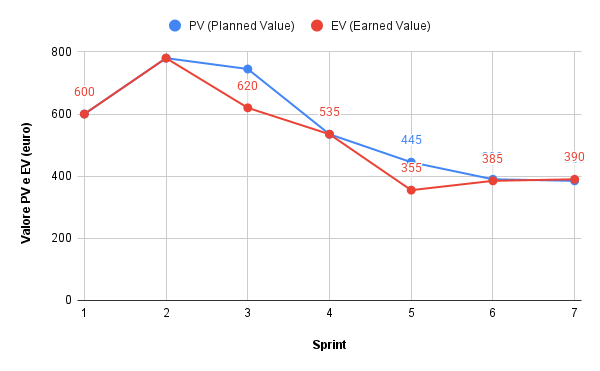
\includegraphics[width=0.75\textwidth]{../graficiMetriche/PV.png}
    \caption{Andamento e confronto di PV e EV nella fase RTB}
\end{figure}

\textbf{RTB:} Dal confronto tra le curve di Planned Value (costo pianificato) ed Earned Value (valore prodotto), emerge una flessione dell'EV durante lo \gls{Sprint} 3 e lo \gls{Sprint} 5 a causa della ridotta disponibilità oraria durante il periodo natalizio e per gli esami invernali.

Tuttavia, analizzando anche l'Actual Cost (AC, non rappresentato in figura ma rendicontato nei consuntivi), emerge che i costi effettivi si sono mantenuti sempre allineati o inferiori all'EV: questo dimostra che le spese sono state costantemente sotto controllo e proporzionate al lavoro realmente svolto, senza alcuno spreco. Durante gli \gls{Sprint} 6 e 7 il team ha incrementato la produttività, riportando l'EV ad allinearsi al PV e chiudendo la fase senza debiti temporali e con un risparmio effettivo (AC $<$ PV).

\newpage
\subsubsection{Schedule Performance Index (SPI)}
% [GRAFICO DELL'SPI]
\begin{figure}[H]
    \centering
    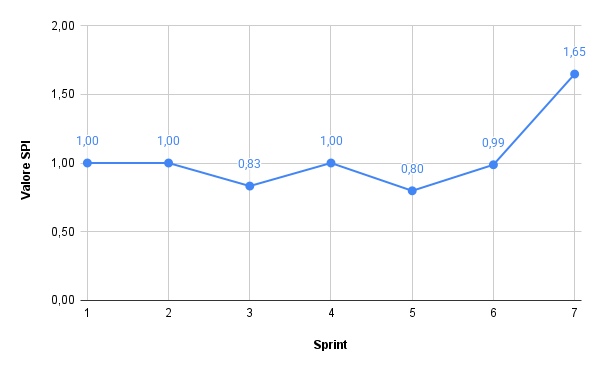
\includegraphics[width=0.75\textwidth]{../graficiMetriche/SPI.png}
    \caption{Andamento dello Schedule Performance Index (SPI) nella fase RTB}
\end{figure}

\textbf{RTB:} L'indice di efficienza della schedulazione (SPI) evidenzia visibilmente l'impatto della sessione d'esami, toccando un picco negativo di 0.83 nello \gls{Sprint} 3 e di 0.80 nello \gls{Sprint} 5. Questo scostamento si è tradotto in una Schedule Variance (SV) negativa, che ha toccato un picco di -125 € nello \gls{Sprint} 3.

Tuttavia, la ridistribuzione dei carichi di lavoro ha permesso di recuperare il gap già negli \gls{Sprint} successivi (4 e 6) e di chiudere lo \gls{Sprint} 7 in perfetto orario (SPI a 1.65) e con un saldo temporale tornato in positivo. L'andamento a "V" del grafico dimostra un'ottima capacità di reazione del team agli imprevisti temporali. L'obiettivo del team è rendere l'indice più stabile nella prossima fase di PB attraverso una migliore pianificazione delle attività.

\newpage
\subsubsection{Cost Performance Index (CPI)}
% [GRAFICO DEL CPI]
\begin{figure}[H]
    \centering
    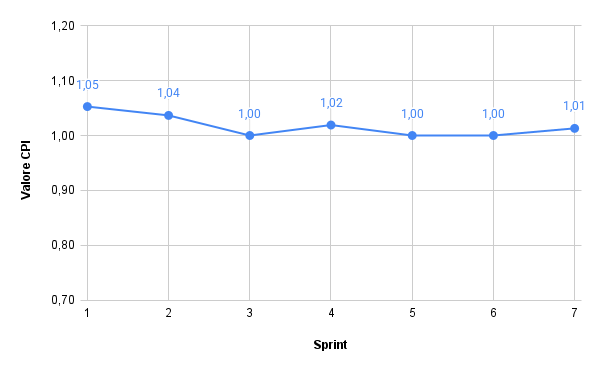
\includegraphics[width=0.75\textwidth]{../graficiMetriche/CPI.png}
    \caption{Andamento del Cost Performance Index (CPI) nella fase RTB}
\end{figure}

\textbf{RTB:} L'indice di efficienza dei costi (CPI) mostra un andamento eccellente, mantenendosi costantemente attorno al valore 1.0 o superiore. Ciò significa che per ogni euro speso dal progetto, il valore prodotto è stato pari o superiore a un euro. Nonostante il ritardo temporale (SPI $<$ 1) negli \gls{Sprint} 3 e 5, il gruppo è stato molto efficiente economicamente: le ore lavorate sono state produttive e non ci sono stati sprechi di risorse o rilavorazioni costose che avrebbero abbassato il CPI.

\newpage
\subsubsection{Cost Variance (CV)}
% [GRAFICO DELLA CV]
\begin{figure}[H]
    \centering
    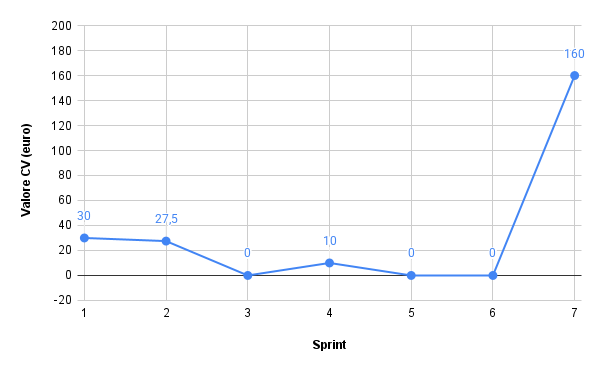
\includegraphics[width=0.75\textwidth]{../graficiMetriche/CV.png}
    \caption{Andamento della Cost Variance (CV) nella fase RTB}
\end{figure}

\textbf{RTB:} La varianza dei costi (CV), calcolata come differenza tra Earned Value e Actual Cost ($EV - AC$), si è mantenuta positiva o prossima allo zero per tutta la durata della fase. Questo indicatore conferma che il gruppo non ha mai speso più del valore generato. Al termine della RTB, il risparmio cumulato è pari a 227,50 €, garantendo al progetto un prezioso margine di sicurezza economico da investire nella successiva fase di Product Baseline.

\newpage
\subsubsection{Requirements Stability Index (RSI)}
% [GRAFICO RSI]
\begin{figure}[H]
    \centering
    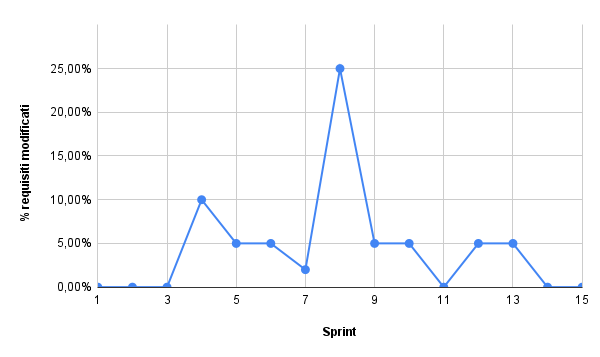
\includegraphics[width=0.75\textwidth]{../graficiMetriche/RSI.png}
    \caption{Andamento del Requirements Stability Index (RSI) nella fase RTB}
\end{figure}

\textbf{RTB:} L'indice di stabilità dei requisiti ha subito alcune variazioni in particolare durante lo \gls{Sprint} 4 e 5. A seguito del colloquio di \gls{verifica} con il prof. Cardin, il gruppo ha dovuto apportare correzioni e raffinamenti ai casi d'uso e ai requisiti precedentemente individuati. Negli ultimi \gls{sprint} (\gls{Sprint} 6), con il consolidamento dell'architettura per il PoC, l'indice si è stabilizzato, indicando che il perimetro del progetto è ora ben definito.

\newpage
\subsubsection{Rischi Non Calcolati (RNC)}
% [GRAFICO RNC]
\begin{figure}[H]
    \centering
    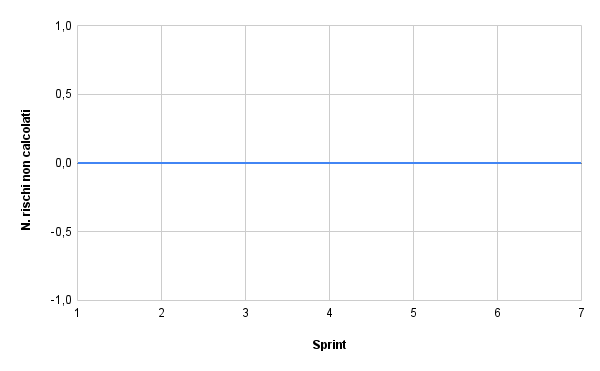
\includegraphics[width=0.75\textwidth]{../graficiMetriche/RNC.png}
    \caption{Numero di rischi non calcolati (RNC) nella fase RTB}
\end{figure}

\textbf{RTB:} Durante la fase RTB, il numero di rischi imprevisti è stato pari a zero (o molto basso). Le principali criticità riscontrate, come la ridotta disponibilità dovuta agli esami (RO-1) e le difficoltà di apprendimento delle tecnologie LLM (RT-1), erano state correttamente previste e mitigate. Il gruppo può ritenersi soddisfatto della capacità di previsione e gestione dei rischi.

\newpage
\subsubsection{Metriche Soddisfatte (MS)}
% [GRAFICO MS]
\begin{figure}[H]
    \centering
    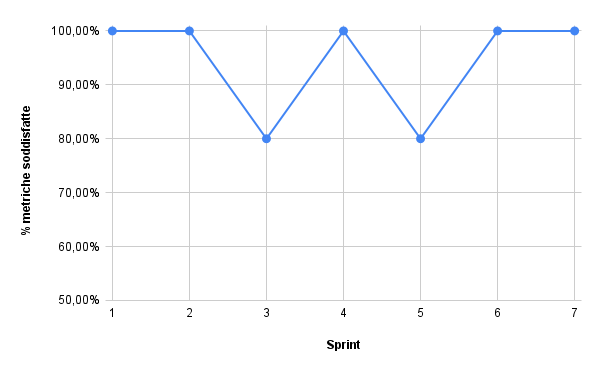
\includegraphics[width=0.75\textwidth]{../graficiMetriche/MS.png}
    \caption{Percentuale delle metriche soddisfatte (MS) nella fase RTB}
\end{figure}

\textbf{RTB:} La percentuale complessiva di metriche soddisfatte ha registrato due flessioni (attorno all'80\%) in corrispondenza degli \gls{Sprint} 3 e 5, principalmente a causa degli sforamenti temporali (SPI < 0.90). Tuttavia, la tenuta impeccabile delle metriche economiche (CPI, CV sempre ottimali) e il recupero finale hanno permesso di chiudere la fase con il 100\% degli indicatori in stato accettabile o ottimale. Il processo adottato è pertanto ritenuto maturo e validato.

\end{document}
